\documentclass[10pt,a4paper]{article}
\usepackage[papersize={596pt,842pt},margin=0.5in]{geometry}
\usepackage{paracol}
\usepackage{fancyhdr}
\usepackage{listings}
\usepackage{graphicx}
\usepackage{amsmath,amssymb}
\usepackage[T1]{fontenc}
\usepackage{mathptmx}
\usepackage{courier}
\usepackage{xcolor}
\definecolor{codekw}{rgb}{0.10,0.35,0.65}     % vivid blue for keywords
\definecolor{codestr}{rgb}{0.70,0.40,0.15}     % warm orange-brown for strings (VS Code style)
\definecolor{codecmt}{rgb}{0.35,0.35,0.35}     % medium gray for comments
\definecolor{codenum}{rgb}{0.10,0.55,0.10}     % green for numbers (VS Code style)
\definecolor{codepre}{rgb}{0.55,0.18,0.60}     % purple for preprocessor
\definecolor{codetype}{rgb}{0.15,0.58,0.55}    % teal for C++ types (VS Code style)
\usepackage{caption}
\usepackage{tikz}

\setlength{\columnsep}{39pt}
\setlength{\columnseprule}{0.4pt}

\pagestyle{fancy}
\fancyhf{}
\renewcommand{\headrulewidth}{0.8pt}
\fancyhead[L]{\vspace*{15pt}\textbf{JUST\_ORIONS} - Jashore University of Science and Technology}
\fancyhead[R]{\thepage}
\fancyfoot{}

\lstset{
  language=C++,
  basicstyle=\ttfamily\footnotesize,
  keywordstyle=\color{codekw},
  stringstyle=\color{codestr},
  commentstyle=\color{codecmt},
  numberstyle=\color{codenum},
  identifierstyle=\color{black},
  directivestyle=\color{codepre},
  emph={int,long,double,char,void,bool,short,float,unsigned,
    signed,size_t,ssize_t,int8_t,int16_t,int32_t,int64_t,
    uint8_t,uint16_t,uint32_t,uint64_t,__int128_t,
    int128_t,uint128_t,vector,map,set,pair,string,queue,
    stack,deque,list,unordered_map,unordered_set,
    multiset,multimap,priority_queue,tuple,optional,
    variant,array,complex,valarray,initializer_list,
    istream,ostream,ifstream,ofstream,stringstream,
    istringstream,ostringstream,auto,decltype,nullptr_t,
    mt19937,mt19937_64,uniform_int_distribution,
    pb_ds,gnu_pbds,tree,null_type,rb_tree_tag,
    tree_order_statistics_node_update,ordered_set,OS,
    gp_hash_table,chash},
  emphstyle=\color{codetype},
  morekeywords={emplace_back,push_back,make_pair,iota,
    fill,upper_bound,lower_bound,binary_search,swap,
    insert,erase,find,count,begin,end,size,empty,
    clear,assign,push,pop,top,front,back,sort,
    reverse,accumulate,adjacent_find,all_of,any_of,
    binary_search,copy,count_if,equal_range,fill_n,
    find_if,for_each,generate,includes,inplace_merge,
    is_heap,is_sorted,iter_swap,lexicographical_compare,
    lower_bound,make_heap,max_element,merge,min_element,
    next_permutation,nth_element,partial_sort,partition,
    pop_heap,prev_permutation,push_heap,random_shuffle,
    remove,remove_if,replace,replace_if,reverse_copy,
    rotate,search,set_difference,set_intersection,
    set_symmetric_difference,set_union,shuffle,sort_heap,
    stable_partition,stable_sort,swap_ranges,transform,
    unique,unique_copy,resize,reserve,shrink_to_fit,
    data,at,substr,compare,append,assign,replace,find,
    rfind,find_first_of,find_last_of,npos},
  keywordstyle=\color{codekw},
  breaklines=true,
  breakatwhitespace=false,
  frame=none,
  columns=fullflexible,
  keepspaces=true,
  showspaces=false,
  showstringspaces=false,
  aboveskip=4pt,
  belowskip=4pt,
  lineskip=1pt,
  upquote=true,
  tabsize=2,
}

\setlength{\parskip}{6pt}
\setlength{\parindent}{0pt}

\linespread{1.2}

\begin{document}

\columnratio{0.5}
\begin{paracol}{2}

\textbf{\Large Sublime build(linux):}
\begin{lstlisting}
{
  "shell": true,
  "cmd": "g++ -std=c++17 '${file}' -o
  '${file_path}/${file_base_name}' &&
  '${file_path}/${file_base_name}' < input.txt >
  output.txt",
  "working_dir": "${file_path}",
  "selector": "source.cpp"
}
\end{lstlisting}

\textbf{Windows:}
\begin{lstlisting}
{
  "cmd": ["g++.exe",
  "-std=c++17", "${file}",
  "-o",
  "${file_base_name}.exe",
  "&&" ,
  "${file_base_name}.exe<input.txt>output.txt"],
  "shell":true,
  "working_dir":"$file_path",
  "selector":"source.cpp"
}
\end{lstlisting}

\textbf{Nothing}
\begin{lstlisting}
#pragma GCC optimize("Ofast")
ios_base::sync_with_stdio(false), cin.tie(NULL),
cout.tie(NULL);
#ifndef ONLINE_JUDGE
freopen("input.txt", "r",
stdin),freopen("output.txt", "w", stdout);
#endif
auto rd = [](){ ll x; cin >> x; return x; };
#define dbg(x) cerr << "[" #x "] = " << (x) << "\n"
mt19937_64 rnd((unsigned
int)chrono::steady_clock::now().time_since_epoch
().count());
int64_t Random(int64_t l, int64_t r) { return (l +
(rnd() % (r - l + 1))); }
\end{lstlisting}

$\sum$ coprime of $(x) = (x \cdot \phi(x))/2$.

\textbf{PBDS}
\begin{lstlisting}
#include <ext/pb_ds/assoc_container.hpp>
#include <ext/pb_ds/tree_policy.hpp>
using namespace __gnu_pbds;
template <class T>
using OS = tree<T, null_type, less<T>,
rb_tree_tag,
tree_order_statistics_node_update>;
// to erase in multiset-> less_equal<T> and
// s.erase(s.find_by_order(s.order_of_key(x)))
// ll idx = s.order_of_key(x)
// if(idx == s.size()) -> no lower_bound
// else lb = *s.find_by_order(idx) // as
// 0-indexing
// idx-1 will give highest value which is strictly
// less than x
// for upper_bound->do the same with (x+1)
\end{lstlisting}

\textit{Custom cmp pbds:}

\begin{lstlisting}
struct cmp {bool operator() (const int &a,const int
&b){return a <= b;}};
typedef
tree<int,null_type,cmp,rb_tree_tag,tree_order_s
tatistics_node_update> ordered_set;
\end{lstlisting}

\switchcolumn

\textbf{\textit{GP Hash Table}}
\begin{lstlisting}
struct chash {
  static uint64_t splitmix64(uint64_t x)
  {
    x += 0x9e3779b97f4a7c15;
    x = (x ^ (x >> 30)) * 0xbf58476d1ce4e5b9;
    x = (x ^ (x >> 27)) * 0x94d049bb133111eb;
    return x ^ (x >> 31);
  }
  int operator()(int x) const
  {
    static const uint64_t FIXED_RANDOM =
    chrono::steady_clock::now().time_since_epoch()
    .count();
    return splitmix64(x + FIXED_RANDOM);
  }
};
gp_hash_table<ll, ll, chash> mp;
\end{lstlisting}

\textbf{DSU}
\begin{lstlisting}
struct DSU{
  vector<int> p, rank, setSize;
  int numSets;
  DSU(int N)
  {
    p.assign(N, 0);
    iota(p.begin(), p.end(), 0);
    rank.assign(N, 0), setSize.assign(N, 1);
    numSets = N;
  }
  int findSet(int i) { return (p[i] == i) ? i : (p[i] =
  findSet(p[i])); }
  bool isSameSet(int i, int j) { return findSet(i) ==
  findSet(j); }
  int numDisjointSets() { return numSets; }
  int sizeOfSet(int i) { return setSize[findSet(i)]; }
  void unionSet(int i, int j)
  {
    if (isSameSet(i, j))
      return;
    int x = findSet(i), y = findSet(j);
    if (rank[x] > rank[y])
      swap(x, y);
    p[x] = y;
    if (rank[x] == rank[y])
      ++rank[y];
    setSize[y] += setSize[x];
    --numSets;
  }
};
\end{lstlisting}

\switchcolumn

\textbf{Persistent Segment Tree}
\begin{lstlisting}
struct PST {
  struct Node { int l, r, val; };
  vector<Node> t;
  int T = 0;
  PST(int max_nodes) { // estimate 20 * n for
  // max_nodes
    t.resize(max_nodes);
  }
  int build(int b, int e) {
    int cur = T++;
    if (b == e) return cur;
    int m = (b + e) / 2;
    t[cur].l = build(b, m);
    t[cur].r = build(m + 1, e);
    return cur;
  }
  int update(int pre, int b, int e, int i, int v) {
    int cur = T++;
    t[cur] = t[pre];
    if (b == e) {
      t[cur].val += v;
      return cur;
    }
    int m = (b + e) / 2;
    if (i <= m) t[cur].l = update(t[pre].l, b, m, i,
    v);
    else t[cur].r = update(t[pre].r, m + 1, e, i, v);
    t[cur].val = t[t[cur].l].val + t[t[cur].r].val;
    return cur;
  }
  int query(int pre, int cur, int b, int e, int k) {
    if (b == e) return b;
    int cnt = t[t[cur].l].val - t[t[pre].l].val;
    int m = (b + e) / 2;
    if (cnt >= k) return query(t[pre].l, t[cur].l, b,
    m, k);
    return query(t[pre].r, t[cur].r, m + 1, e, k - cnt);
  }
};
int main() {
  ios::sync_with_stdio(0); cin.tie(0);
  int n, q;
  cin >> n >> q;
  vector<int> a(n + 1), root(n + 1), V;
  map<int, int> comp;
  for (int i = 1; i <= n; i++) cin >> a[i],
  comp[a[i]];
  int id = 0;
  V.resize(comp.size() + 1);
  for (auto& [x, _] : comp) comp[x] = ++id, V[id]
  = x;
  PST pst(20 * (n + 1)); // Allocate enough space
  root[0] = pst.build(1, id);
  for (int i = 1; i <= n; i++)
  root[i] = pst.update(root[i - 1], 1, id,
  comp[a[i]], 1);
  while (q--) {
    int l, r, k;
    cin >> l >> r >> k;
    cout << V[pst.query(root[l - 1], root[r], 1, id,
    k)] << '\n';
  }
  return 0;
}
\end{lstlisting}
%the code returns k-th number in a range l to r if
%the range were sorted
\begin{lstlisting}
int V[N], root[N], a[N];
int32_t main() {
  map<int, int>mp;
  int n, q;
  cin >> n >> q;
  for(int i = 1; i <= n; i++) cin >> a[i], mp[a[i]];
  int c = 0;
  for(auto x : mp) mp[x.first] = ++c, V[c] = x.first;
  root[0] = t.build(1, n);
  for(int i = 1; i <= n; i++) {
    root[i] = t.upd(root[i - 1], 1, n, mp[a[i]], 1);
  }
  while(q--) {
    int l, r, k;
    cin >> l >> r >> k;
    cout << V[t.query(root[l - 1], root[r], 1, n, k)]
    << '\n';
  }
  return 0;
}
\end{lstlisting}

\switchcolumn

\textbf{Fenwick Tree}
Point update and range query.
\begin{lstlisting}
template<typename T>
struct BIT {
  int n;
  vector<T> bit;
  BIT(int n = 0) { init(n); }
  void init(int n_) { n = n_; bit.assign(n + 1, 0); }
  void add(int i, T v) { for (; i <= n; i += i & -i)
    bit[i] += v; }
  T sum(int i) { T r = 0; for (; i > 0; i -= i & -i) r
    += bit[i]; return r; }
  T sum(int l, int r) { return sum(r) - sum(l - 1); }
};
\end{lstlisting}
Usage: \texttt{BIT<ll> fenw(5);}

\textit{//Fenwick 2D}
\begin{lstlisting}
struct BIT2D {
  int n, m;
  vector<vector<ll>> bit;
  BIT2D(int n, int m): n(n), m(m) {
    bit.assign(n + 1, vector<ll>(m + 1, 0));
  }
  void add(int x, int y, ll val) {
    for (int i = x; i <= n; i += i & -i)
      for (int j = y; j <= m; j += j & -j)
        bit[i][j] += val;
  }
  ll sum(int x, int y) {
    ll res = 0;
    for (int i = x; i > 0; i -= i & -i)
      for (int j = y; j > 0; j -= j & -j)
        res += bit[i][j];
    return res;
  }
  ll query(int x1, int y1, int x2, int y2) {
    return sum(x2, y2) - sum(x1 - 1, y2) - sum(x2,
    y1 - 1) + sum(x1 - 1, y1 - 1);
  }
};
\end{lstlisting}
\begin{lstlisting}
BIT2D fenw2(4, 4);
fenw2.add(1, 1, 5);
fenw2.add(3, 2, 7);
cout << fenw2.query(1, 1, 3, 3) << "\n"; // sum
// inside rectangle [(1,1)-(3,3)]
\end{lstlisting}

Range update and range query.
\begin{lstlisting}
using ll = long long;
ll bit1[200005] ,bit2[200005],n,m;
void update(ll bit[],ll i,ll val){
  for(;i<=n;i+=(i&(-i))){
    bit[i]+=val;
  }
}
void range_update(ll l, ll r,ll val){
  update(bit1,l,val);
  update(bit1,r+1,-val);
  update(bit2,l,val*(l-1));
  update(bit2,r+1,-(r*val));
}
ll sum(ll bit[],ll i){
  ll re = 0;
  for(;i>0;i-=(i&(-i))){
    re+=bit[i];
  }
  return re;
}
ll prefix_sum(ll i){
  return sum(bit1,i)*i-sum(bit2,i);
}
ll range_sum(ll l,ll r){
  return prefix_sum(r)-prefix_sum(l-1);
}
\end{lstlisting}
\texttt{range\_update(l,r,val);}\\
\texttt{range\_sum(l,r);}

\switchcolumn

\textbf{Sparse Table}
Max/Min/GCD Query
\begin{lstlisting}
struct SparseTable {
  SparseTable(vector<int>& data)
  {
    int n = data.size();
    int maxLog = log2(n) + 1;
    table.assign(n, vector<int>(maxLog));
    for (int i = 0; i < n; ++i) {
      table[i][0] = data[i];
    }
    for (int j = 1; (1 << j) <= n; ++j) {
      for (int i = 0; (i + (1 << j) - 1) < n; ++i) {
        table[i][j] = max(table[i][j - 1], table[i +
        (1 << (j - 1))][j - 1]);
      }
    }
  }
  int query(int L, int R)
  {
    int j = log2(R - L + 1);
    return max(table[L][j], table[R - (1 << j) +
    1][j]);
  }
  vector<vector<int>> table;
};
\end{lstlisting}
\begin{lstlisting}
int main()
{
  vector<int> data = { 1, 3, 2, 7, 9, 11, 3, 5, 6, 8 };
  SparseTable st(data);
  cout << "Max in range [1, 4]: " << st.query(1, 4)
  << endl;
}
\end{lstlisting}

\textbf{Sparse Table 2D} (up to 500 x 500 is safe)
\begin{lstlisting}
struct SparseTable2D {
  static const int LG = 10;
  int n, m;
  vector<vector<int>> a;
  vector<int> lg2;
  vector<vector<vector<vector<int>>>> st;
  SparseTable2D(int n, int m) : n(n), m(m) {
    a.assign(n, vector<int>(m, 0));
    lg2.resize(max(n, m) + 1, 0);
    for (int i = 2; i <= max(n, m); i++) lg2[i] =
    lg2[i >> 1] + 1;
    st.assign(n, vector<vector<vector<int>>>(m,
    vector<vector<int>>(LG, vector<int>(LG,
    0))));
  }
  void set_val(int i, int j, int val) { a[i][j] = val; }
  void build() {
    for (int i = 0; i < n; i++)
      for (int j = 0; j < m; j++)
        st[i][j][0][0] = a[i][j];
    for (int a = 0; a < LG; a++) {
      for (int b = 0; b < LG; b++) {
        if (a + b == 0) continue;
        for (int i = 0; i + (1 << a) <= n; i++) {
          for (int j = 0; j + (1 << b) <= m; j++) {
            if (!a)
              st[i][j][a][b] = max(st[i][j][a][b-1],
              st[i][j + (1 << (b - 1))][a][b - 1]);
            else
              st[i][j][a][b] = max(st[i][j][a-1][b],
              st[i + (1 << (a - 1))][j][a - 1][b]);
          }
        }
      }
    }
  }
  int query(int x1, int y1, int x2, int y2) {
    int a = lg2[x2 - x1 + 1], b = lg2[y2 - y1 + 1];
    int m1 = max(st[x1][y1][a][b], st[x2 - (1 << a)
    + 1][y1][a][b]);
    int m2 = max(st[x1][y2 - (1 << b) + 1][a][b],
    st[x2 - (1 << a) + 1][y2 - (1 << b) + 1][a][b]);
    return max(m1, m2);
  }
};
\end{lstlisting}
\begin{lstlisting}
// st.set_val(i, j, grid[i][j]);
// st.build(); // st.query(0, 0, 1, 2); // max in
// submatrix [(0,0) to (1,2)]
\end{lstlisting}

\switchcolumn

\textbf{Merge Sort Tree}
\begin{lstlisting}
struct MergeSortTree {
  vector<vector<int>> tree;
  vector<int> arr;
  int n;
  MergeSortTree(vector<int>& a)
  {
    arr = a, n = a.size();
    tree.resize(4 * n);
    build(1, 0, n - 1);
  }
  void build(int node, int l, int r)
  {
    if (l == r) {
      tree[node].push_back(arr[l]);
      return;
    }
    int mid = (l + r) / 2;
    build(node * 2, l, mid), build(node * 2 + 1,
    mid + 1, r);
    merge(tree[node * 2].begin(), tree[node *
    2].end(), tree[node * 2 + 1].begin(), tree[node * 2
    + 1].end(), back_inserter(tree[node]));
  }
  int query(int node, int l, int r, int ql, int qr, int
  k)
  {
    if (l > qr || r < ql)
      return 0;
    if (l >= ql && r <= qr) {
      int hi = tree[node].size() - 1, lo = 0, ind =
      -1;
      // while (hi >= lo) { } // Modify your
      // function here
      return ind;
    }
    int mid = (l + r) / 2;
    return query(node * 2, l, mid, ql, qr, k) +
    query(node * 2 + 1, mid + 1, r, ql, qr, k);
  }
};
\end{lstlisting}

Find the number of distinct elements in a range.
\begin{lstlisting}
void merge(vector<int> tree[], int treeNode)
{
  int len1 = tree[2 * treeNode].size();
  int len2 = tree[2 * treeNode + 1].size();
  int index1 = 0, index2 = 0;
  while (index1 < len1 && index2 < len2) {
    if (tree[2 * treeNode][index1]
    > tree[2 * treeNode + 1][index2]) {
      tree[treeNode].push_back(
      tree[2 * treeNode + 1][index2]);
      index2++;
    }
    else {
      tree[treeNode].push_back(
      tree[2 * treeNode][index1]);
      index1++;
    }
  }
  while (index1 < len1) {
    tree[treeNode].push_back(
    tree[2 * treeNode][index1]);
    index1++;
  }
  while (index2 < len2) {
    tree[treeNode].push_back(
    tree[2 * treeNode + 1][index2]);
    index2++;
  }
  return;
}
\end{lstlisting}

\begin{lstlisting}
void build(vector<int> tree[], int* arr, int start,
int end,
int treeNode)
{
  if (start == end) {
    tree[treeNode].push_back(arr[start]);
    return;
  }
  int mid = (start + end) / 2;
  build(tree, arr, start, mid, 2 * treeNode);
  build(tree, arr, mid + 1, end, 2 * treeNode + 1);
  merge(tree, treeNode);
  return;
}
\end{lstlisting}

\switchcolumn

\begin{lstlisting}
int query(vector<int> tree[], int treeNode, int
start,
int end, int left, int right)
{
  if (start > right || end < left) {
    return 0;
  }
  if (start >= left && end <= right) {
    return tree[treeNode].end()
    - upper_bound(tree[treeNode].begin(),
    tree[treeNode].end(), right);
  }
  int mid = (start + end) / 2;
  int op1 = query(tree, 2 * treeNode, start, mid,
  left,
  right);
  int op2 = query(tree, 2 * treeNode + 1, mid + 1,
  end,
  left, right);
  return op1 + op2;
}
int main()
{
  int n; cin >> n;
  int arr[n];
  for(int i=0;i<n;i++) cin >> arr[i];
  int next_right[n];
  vector<int> tree[4 * n];
  unordered_map<int, int> ump;
  for (int i = n - 1; i >= 0; i--) {
    if (ump[arr[i]] == 0) {
      next_right[i] = n;
      ump[arr[i]] = i;
    }
    else {
      next_right[i] = ump[arr[i]];
      ump[arr[i]] = i;
    }
  }
  build(tree, next_right, 0, n - 1, 1);
  int q; cin >> q;
  while(q--){
    int l, r; cin >> l >> r;
    l-- , r--;
    cout << query(tree,1,0,n-1,l,r) << "\n";
  }
  return 0;
}
\end{lstlisting}

\textbf{Kth smallest value in a range (SegTree)}
\begin{lstlisting}
#define N (int)1e5
vector<int> seg[N];
void build(int ci, int st, int end,
pair<int, int>* B)
{
  if (st == end) {
    seg[ci].push_back(B[st].second);
    return;
  }
  int mid = (st + end) / 2;
  build(2 * ci + 1, st, mid, B);
  build(2 * ci + 2, mid + 1, end, B);
  merge(seg[2 * ci + 1].begin(), seg[2 * ci +
  1].end(),
  seg[2 * ci + 2].begin(), seg[2 * ci + 2].end(),
  back_inserter(seg[ci]));
}
\end{lstlisting}

\switchcolumn

\begin{lstlisting}
int query(int ci, int st, int end,
int l, int r, int k)
{
  if (st == end)
    return seg[ci][0];
  int p = upper_bound(seg[2 * ci + 1].begin(),
  seg[2 * ci + 1].end(), r)
  - lower_bound(seg[2 * ci + 1].begin(),
  seg[2 * ci + 1].end(), l);
  int mid = (st + end) / 2;
  if (p >= k)
    return query(2 * ci + 1, st, mid, l, r, k);
  else
    return query(2 * ci + 2, mid + 1, end, l, r, k-p);
}
int main()
{
  int arr[] = { 3, 1, 5, 2, 4, 7, 8, 6 };
  int n = sizeof(arr) / sizeof(arr[0]);
  pair<int, int> B[n];
  for (int i = 0; i < n; i++) {
    B[i] = { arr[i], i };
  }
  sort(B, B + n);
  build(0, 0, n - 1, B);
  cout << "3rd smallest element in range 3 to 7 is:
  "
  << arr[query(0, 0, n - 1, 2, 6, 3)] << "\n";
}
\end{lstlisting}

\textbf{Treap}
\begin{lstlisting}
mt19937
rnd(chrono::steady_clock::now().time_since_epoch
().count());
struct Node {
  int64_t prior, data, sum, toProp;
  int size; bool rev; Node *l, *r;
  Node(int64_t val) {
    prior = rnd(), data = sum = val;
    size = 1; rev = toProp = 0;
    l = r = nullptr;
  }
};
struct Treap {
  Node *root;
  Treap() : root(nullptr) {}
  int size(Node *&t) { return t ? t -> size : 0; }
  int64_t sum(Node *&t) { return t ? t -> sum : 0;
  }
  void update(Node *&t) {
    if (!t) return;
    t -> size = size(t -> l) + size(t -> r) + 1;
    t -> sum = t -> data + t -> size * t -> toProp;
    if (t -> l) t -> sum += t -> l -> sum + t -> l ->
    size * t -> l -> toProp;
    if (t -> r) t -> sum += t -> r -> sum + t -> r ->
    size * t -> r -> toProp;
  }
  void push(Node *&t) {
    if (!t) return;
    if (t -> rev) {
      t -> rev = false; swap(t -> l, t -> r);
      if (t -> l) t -> l -> rev ^= true;
      if (t -> r) t -> r -> rev ^= true;
    }
    if (t -> toProp) {
      t -> data += t -> toProp;
      if (t -> l) t -> l -> toProp += t -> toProp;
      if (t -> r) t -> r -> toProp += t -> toProp;
      t -> toProp = 0;
    }
  }
\end{lstlisting}

\switchcolumn

\begin{lstlisting}
  void split(Node *t, Node *&l, Node *&r, int key,
  int add = 0) {
    if (!t) l = r = nullptr;
    else {
      push(t);
      if (key <= add + size(t -> l)) split(t -> l, l,
      t -> l,
      key, add), r = t;
      else split(t -> r, t -> r, r, key,
      add + 1 + size(t ->
      l)), l = t;
      update(t);
    }
  }
  void merge(Node *&t, Node *l, Node *r) {
    push(l), push(r);
    if (!l || !r) t = l ? l : r;
    else if (l -> prior > r -> prior) merge(l -> r, l ->
    r, r), t = l;
    else merge(r -> l, l, r -> l), t = r;
    update(t);
  }
  void insert(Node *&t, int key, int64_t val) {
    Node *left, *right; split(t, left, right, key);
    merge(left, left, new Node(val)), merge(t, left,
    right);
  }
  void reverse(Node *&t, int l, int r) {
    Node *left, *mid, *right;
    split(t, left, right, l), split(right, mid, right, r - l
    + 1);
    assert(mid); mid -> rev ^= true;
    merge(t, left, mid), merge(t, t, right);
  }
  int erase(Node *&t, int key) {
    assert(size(t) > key); Node *left, *mid, *right;
    split(t, left, right, key),
    split(right, mid, right, 1);
    merge(t, left, right); int ret = mid -> data;
    delete mid; return ret;
  }
  int64_t query_sum(Node *&t, int l, int r) {
    Node *left, *mid, *right;
    split(t, left, right, l), split(right, mid,
    right, r - l + 1);
    int64_t ret = mid -> sum; merge(t, left, mid),
    merge(t, t, right);
    return ret;
  }
  void rangeAdd(Node *&t, int l, int r, int64_t val)
  {
    Node *left, *mid, *right;
    split(t, left, right, l), split(right, mid,
    right, r - l + 1);
    mid -> toProp += val; merge(t, left, mid),
    merge(t, t, right);
  }
  void set(Node *&t, int p, int64_t val) {
    Node *left, *mid, *right;
    split(t, left, right, p),
    split(right, mid, right, 1);
    merge(t, left, new Node(val)),
    merge(t, t, right);
  }
};
\end{lstlisting}

\switchcolumn

\textbf{Graph Condense}
// Implements Kosaraju's algorithm to find all
// Strongly Connected Components (SCCs).
\begin{lstlisting}
vector<bool>visited;
void dfs(int v, vector<vector<int>> const& g,
vector<int>& output) {
  visited[v] = true;
  for (auto u : g[v])
    if (!visited[u])
      dfs(u, g, output);
  output.push_back(v);
}
void strongly_connected_components(
  vector<vector<int>> const& g,
  vector<vector<int>>& components,
  vector<vector<int>>& g_cond,
  vector<int>& roots
){
  int n = sz(g);
  components.clear(); g_cond.clear();
  vector<int> order;
  visited.assign(n, false);
  for (int i = 0; i < n; ++i)
    if (!visited[i])
      dfs(i, g, order);
  vector<vector<int>> g_rev(n);
  for (int v = 0; v < n; ++v)
    for (int u : g[v])
      g_rev[u].push_back(v);
  visited.assign(n, false);
  reverse(order.begin(), order.end());
  roots.assign(n, -1);
  int component_id = 0;
  for (int v : order) {
    if (!visited[v]) {
      vector<int> component;
      dfs(v, g_rev, component);
      for (int u : component)
        roots[u] = component_id;
      components.push_back(component);
      component_id++;
    }
  }
  g_cond.assign(component_id, {});
  for (int v = 0; v < n; ++v) {
    for (int u : g[v]) {
      if (roots[v] != roots[u]) {
        g_cond[roots[v]].push_back(roots[u]);
      }
    }
  }
}
\end{lstlisting}

\textbf{Articulation Points and Bridges in Graph}
\begin{lstlisting}
vector<int> dfs_num, dfs_low, dfs_parent;
vector<bool>articulation_vertex;
int dfsNumberCounter, dfsRoot, rootChildren;
vector<pair<int,int>>bridges;
const int UNVISITED = -1;
void articulationPointAndBridge(int u)
{
  dfs_num[u] = dfsNumberCounter++;
  dfs_low[u] = dfs_num[u];
  for (auto &[v, w] : g[u])
  {
    if (dfs_num[v] == UNVISITED)
    {
      dfs_parent[v] = u;
      if (u == dfsRoot)
        ++rootChildren;
      articulationPointAndBridge(v);
      if (dfs_low[v] >= dfs_num[u])
        articulation_vertex[u] = true;
      if (dfs_low[v] > dfs_num[u])
        bridges.push_back({u,v});
      dfs_low[u] = min(dfs_low[u], dfs_low[v]);
    }
    else if (v != dfs_parent[u])
      dfs_low[u] = min(dfs_low[u],
      dfs_num[v]);
  }
}
\end{lstlisting}

\begin{lstlisting}
// inside int main()
bridges.clear();
dfs_num.assign(n, UNVISITED);
dfs_low.assign(n, 0);
dfs_parent.assign(n, -1);
articulation_vertex.assign(n, false);
dfsNumberCounter = 0;
for (int u = 0; u < n; ++u){
  if (dfs_num[u] == UNVISITED)
  {
    dfsRoot = u;
    rootChildren = 0;
    articulationPointAndBridge(u);
    articulation_vertex[dfsRoot] = (rootChildren
    > 1);
  }
}
\end{lstlisting}

\switchcolumn

\textbf{HopcroftKarp}
\begin{lstlisting}
struct HopcroftKarp { // Bipartite Matching
  int n, m;
  vector<vector<int>> g;
  vector<int> dist, pairU, pairV;
  static const int INF = 1e9;
  HopcroftKarp(int n_ = 0, int m_ = 0) {
    n = n_; m = m_;
    g.assign(n, {});
    pairU.assign(n, -1);
    pairV.assign(m, -1);
    dist.assign(n, 0);
  }
  void add_edge(int u, int v) {
    g[u].push_back(v);
  }
  bool bfs() {
    queue<int> q;
    for (int u = 0; u < n; ++u) {
      if (pairU[u] == -1) {
        dist[u] = 0;
        q.push(u);
      } else {
        dist[u] = INF;
      }
    }
    bool foundAug = false;
    while (!q.empty()) {
      int u = q.front(); q.pop();
      for (int v : g[u]) {
        int u2 = pairV[v];
        if (u2 == -1) {
          foundAug = true;
        } else if (dist[u2] == INF) {
          dist[u2] = dist[u] + 1;
          q.push(u2);
        }
      }
    }
    return foundAug;
  }
  bool dfs(int u) {
    for (int v : g[u]) {
      int u2 = pairV[v];
      if (u2 == -1 || (dist[u2] == dist[u] + 1 &&
      dfs(u2))) {
        pairU[u] = v;
        pairV[v] = u;
        return true;
      }
    }
    dist[u] = INF;
    return false;
  }
  int max_matching() {
    int matching = 0;
    while (bfs()) {
      for (int u = 0; u < n; ++u)
        if (pairU[u] == -1 && dfs(u))
          ++matching;
    }
    return matching;
  }
  vector<pair<int,int>> matching_edges() const
  {
    vector<pair<int,int>> res;
    for (int v = 0; v < m; ++v)
      if (pairV[v] != -1)
        res.emplace_back(pairV[v], v);
    return res;
  }
};
\end{lstlisting}

\switchcolumn

\textbf{Dinic's Algorithm(Max Flow)}
\begin{lstlisting}
const int64_t inf = 1LL << 61;
struct Dinic {
  struct edge {
    int to, rev;
    int64_t flow, w;
  };
  int n, s, t;
  vector<int> d;
  vector<int> done;
  vector<vector<edge>> g;
  Dinic() {};
  Dinic(int _n) {
    n = _n + 10, g.resize(n);
  }
  void add_edge(int u, int v, int64_t w) {
    edge a = {v, (int)g[v].size(), 0, w};
    edge b = {u, (int)g[u].size(), 0, 0};
    g[u].push_back(a), g[v].push_back(b);
  }
  bool bfs() {
    d.assign(n, -1), d[s] = 0;
    queue<int> Q;
    Q.push(s);
    while (Q.size()) {
      int u = Q.front(); Q.pop();
      for (auto &e : g[u]) {
        int v = e.to;
        if (!~d[v] && e.flow < e.w) d[v] = d[u] + 1,
        Q.push(v);
      }
    }
    return d[t] != -1;
  }
  int64_t dfs(int u, int64_t flow) {
    if (u == t) return flow;
    for (int &i = done[u]; i < (int)g[u].size(); i++) {
      edge &e = g[u][i];
      if (e.w <= e.flow) continue;
      int v = e.to;
      if (d[v] == d[u] + 1) {
        int64_t nw = dfs(v, min(flow, e.w - e.flow));
        if (nw > 0) {
          e.flow += nw;
          g[v][e.rev].flow -= nw;
          return nw;
        }
      }
    }
    return 0;
  }
  int64_t max_flow(int _s, int _t) {
    s = _s, t = _t;
    int64_t flow = 0;
    while (bfs()) {
      done.assign(n, 0);
      while (int64_t nw = dfs(s, inf)) flow += nw;
    }
    return flow;
  }
};
\end{lstlisting}

\switchcolumn

\textbf{Binary Lifting}
\begin{lstlisting}
int up[200001][20];
vector<vector<int>> tree(200001);
void binary_lifting(int src, int par) {
  up[src][0] = par;
  for (int i = 1; i <= 19; i++) {
    if (up[src][i - 1] != -1)
      up[src][i] = up[up[src][i-1]][i-1];
    else
      up[src][i] = -1;
  }
  for (int i = 0; i < tree[src].size(); i++)
    if (tree[src][i] != par)
      binary_lifting(tree[src][i], src);
}
int lift_node(int node, int k) {
  if (node == -1 || k == 0)
    return node;
  for (int i = 19; i >= 0; i--)
    if (k >= (1 << i))
      return lift_node(up[node][i], k-(1<<i));
}
\end{lstlisting}

\textbf{Tree Flattening (Euler Tour)}
\begin{lstlisting}
void eularDFS(ll node, ll par, ll arr[], vector<ll>&
flatTree, vector<ll> tree[], pair<ll, ll>
subTreeRange[], ll& timer)
{
  subTreeRange[node].first = ++timer;
  flatTree.push_back(arr[node]);
  for (auto& child : tree[node])
    if (child != par)
      eularDFS(child, node, arr, flatTree, tree,
      subTreeRange, timer);
  subTreeRange[node].second = timer;
}
void solve() {
  vector<ll> flatTree;
  pair<ll, ll> subTreeRange[n + 1];
  ll timer = -1;
  eularDFS(1, 0, arr, flatTree, tree,
  subTreeRange, timer);
}
\end{lstlisting}

\textbf{Heavy Light Decomposition (HLD on Tree)}
// u to v range query
\begin{lstlisting}
struct HLD {
  int n, cur_pos = 0;
  vector<int> arr, parent, size, depth, heavy,
  head, pos;
  vector<vector<int>> adj;
  FenwickTree segtree;
  HLD(int n) : n(n), arr(n + 1), parent(n + 1),
  size(n + 1), depth(n + 1), heavy(n + 1, 0), head(n +
  1) , pos(n + 1) , adj(n + 1),
  segtree(FenwickTree(n + 1)){ }
  void add_edge(int u, int v) {
    adj[u].push_back(v), adj[v].push_back(u);
  }
  void dfs(int u, int p) {
    parent[u] = p;
    size[u] = 1;
    int max_sz = 0;
    for (int v : adj[u]) {
      if (v == p)
        continue;
      depth[v] = depth[u] + 1;
      dfs(v, u);
      size[u] += size[v];
      if (size[v] > max_sz) {
        max_sz = size[v], heavy[u] = v;
      }
    }
  }
  void decompose(int u, int h) {
    head[u] = h;
    pos[u] = cur_pos++;
    segtree.add(pos[u], arr[u]); // Update
    // Fenwick tree with the +value of arr[u]
    if (heavy[u])
      decompose(heavy[u], h);
    for (int v : adj[u])
      if (v != parent[u] && v != heavy[u])
        decompose(v, v);
  }
\end{lstlisting}

\switchcolumn

\begin{lstlisting}
  int query(int u, int v) { // Range Sum Query
    int res = 0;
    while (head[u] != head[v]) {
      if (depth[head[u]] < depth[head[v]])
        swap(u, v);
      res += segtree.sum(pos[head[u]], pos[u]);
      u = parent[head[u]];
    }
    if (depth[u] > depth[v])
      swap(u, v);
    res += segtree.sum(pos[u], pos[v]);
    return res;
  }
  void addVal(int idx, int delta) {
    segtree.add(pos[idx], delta);
    arr[idx] += delta;
  }
  void editVal(int idx, int value) {
    segtree.add(pos[idx], value - arr[idx]);
    arr[idx] = value;
  }
};
\end{lstlisting}

\textbf{Centroid Decomposition}
\begin{lstlisting}
vector<vector<int>> adj;
vector<bool> is_removed;
vector<int> subtree_size;
int get_subtree_size(int node, int parent = -1) {
  subtree_size[node] = 1;
  for (int child : adj[node]) {
    if (child == parent || is_removed[child]) {
      continue; }
    subtree_size[node] +=
    get_subtree_size(child, node);
  }
  return subtree_size[node];
}
int get_centroid(int node, int tree_size, int parent
= -1) {
  for (int child : adj[node]) {
    if (child == parent || is_removed[child]) {
      continue; }
    if (subtree_size[child] * 2 > tree_size) {
      return get_centroid(child, tree_size, node);
    }
  }
  return node;
}
void build_centroid_decomp(int node = 0) {
  int centroid = get_centroid(node,
  get_subtree_size(node));
  // do something
  is_removed[centroid] = true;
  for (int child : adj[centroid]) {
    if (is_removed[child]) { continue; }
    build_centroid_decomp(child);
  }
}
\end{lstlisting}

\textit{// Ahsan's}
\begin{lstlisting}
int tot = 0;
vector<int> sz(n, 1), removed(n, 0), cenpar(n, -1);
auto dfs_sz = [&](auto &&self, int node, int pr) ->
void {
  tot += 1;
  sz[node] = 1;
  for (auto &son : g[node]) {
    if (son == pr || removed[son]) continue;
    self(self, son, node);
    sz[node] += sz[son];
  }
};
auto find_cen = [&](auto &&self, int node, int pr)
-> int {
  for (auto &son : g[node]) {
    if (son == pr || removed[son]) continue;
    if (sz[son] > tot / 2) return self(self, son, node);
  }
  return node;
};
auto decompose = [&](auto &&self, int node, int
pr) -> void {
  tot = 0;
  dfs_sz(dfs_sz, node, pr);
  int cen = find_cen(find_cen, node, pr);
  removed[cen] = 1;
  cenpar[cen] = pr;
  for (auto &son : g[cen]) {
    if (son == pr || removed[son]) continue;
    self(self, son, cen);
  }
};
decompose(decompose, 0, -1);
\end{lstlisting}

\switchcolumn

\textbf{Tree}
\begin{lstlisting}
vector<vector<int>>t,parents;
vector<int>level;
int mx;
void dfs(int node, int parent, int cLevel){
  level[node] = cLevel;
  parents[0][node] = parent;
  for(auto &x: t[node]){
    if(x!=parent) dfs(x,node, cLevel+1);
  }
}
int kthParent(int a, int k){
  for(int i = 0; i<mx; i++){
    if(a==-1) return a;
    if(k&(1<<i)) a = parents[i][a];
  }
  return a;
}
int lca(int a, int b){
  if(level[a]>level[b]){
    a = kthParent(a, level[a] - level[b]);
  }else{
    b = kthParent(b, level[b] - level[a]);
  }
  if(a==b) return a;
  for(int i = mx-1; i>=0; i--){
    if(parents[i][a]!=parents[i][b]){
      a = parents[i][a];
      b = parents[i][b];
    }
  }
  return parents[0][a];
}
int distance(int a,int b){
  return level[a]+level[b] - 2*level[lca(a,b)];
}
int main(){
  int n;
  cin>>n;
  mx = log2(n)+1;
  //resize and input
  dfs(1,-1,0);
  for(int i = 1; i<mx; i++){
    for(int j = 1; j<=n; j++){
      int prevParent = parents[i-1][j];
      if(prevParent!=-1) parents[i][j] =
      parents[i-1][prevParent];
    }
  }
}
\end{lstlisting}

\textbf{String Double Hashing}
\begin{lstlisting}
ll mod1 = 127657753, mod2 = 987654319, p1 = 31,
p2 = 37;
ll invp1 = ModPow(p1, mod1 - 2, mod1), invp2 =
ModPow(p2, mod2 - 2, mod2);
vector<pair<ll, ll>> pPow(1, {1, 1}), iPow(1, {1,
1});
void genP(ll n) {
  while ((ll)pPow.size() <= n) {
    pPow.push_back({pPow.back().xx * p1 %
    mod1, pPow.back().yy * p2 % mod2});
    iPow.push_back({iPow.back().xx * invp1 %
    mod1, iPow.back().yy * invp2 % mod2});
  }
}
struct Hash {
  int n = 0;
  vector<pair<ll, ll>> sHash;
  void genHash(string& s) {
    sHash.resize(n + 1, {0, 0}); // 0-indexed
    for (int i = 0; i < n; i++) {
      sHash[i + 1].xx = (sHash[i].xx + (s[i] - 'a' +
      1) * pPow[i].xx) % mod1;
      sHash[i + 1].yy = (sHash[i].yy + (s[i] - 'a' +
      1) * pPow[i].yy) % mod2;
    }
  }
  pair<ll, ll> getHash(int l, int r) {
    ll h1 = (sHash[r + 1].xx - sHash[l].xx + mod1)
    % mod1 * iPow[l].xx % mod1;
    ll h2 = (sHash[r + 1].yy - sHash[l].yy + mod2)
    % mod2 * iPow[l].yy % mod2;
    return {h1, h2}; // 0-indexed
  }
  pair<ll, ll> getHash() {
    return sHash[n]; // Get the hash of the whole
    // string
  }
  Hash(string& s) {
    n = s.size();
    genP(n), genHash(s);
  }
};
\end{lstlisting}

\switchcolumn

\textbf{KMP}
\begin{lstlisting}
vector<int> getLps(const string &t) {
  int n = t.size();
  vector<int> pi(n, 0);
  int lps = 0;
  for (int q = 1; q < n; q++) {
    while (lps > 0 && t[lps] != t[q]) {
      lps = pi[lps - 1];
    }
    if (t[lps] == t[q]) {
      lps += 1;
    }
    pi[q] = lps;
  }
  return pi;
}
\end{lstlisting}

\textbf{Z-Algorithm}
\begin{lstlisting}
vector<int> z_function(string& s)
{
  int n = s.size();
  vector<int> z(n);
  z[0] = 0;
  for (int i = 1, l = 0, r = 0; i < n; ++i) {
    if (i <= r)
      z[i] = min(r - i + 1, z[i - l]);
    while (i + z[i] < n && s[z[i]] == s[i + z[i]])
      ++z[i];
    if (i + z[i] - 1 > r)
      l = i, r = i + z[i] - 1;
  }
  return z;
}
\end{lstlisting}

\textbf{Manacher's Algorithm}
\begin{lstlisting}
struct Manacher {
  vector<int> p[2];
  // p[1][i] = (max odd length palindrome
  // centered at i) / 2 [floor division]
  // p[0][i] = same for even, it considers the right
  // center
  // e.g. for s = "abbabba", p[1][3] = 3,
  // p[0][2] = 2
  Manacher(string s) {
    int n = s.size();
    p[0].resize(n + 1);
    p[1].resize(n);
    for (int z = 0; z < 2; z++) {
      for (int i = 0, l = 0, r = 0; i < n; i++) {
        int t = r - i + !z;
        if (i < r) p[z][i] = min(t, p[z][l + t]);
        int L = i - p[z][i], R = i + p[z][i] - !z;
        while (L >= 1 && R + 1 < n && s[L - 1] == s[R
        + 1]) p[z][i]++, L--, R++;
        if (R > r) l = L, r = R;
      }
    }
  }
  bool is_pal(int l, int r) {
    int mid = (l + r + 1) / 2, len = r - l + 1;
    return 2 * p[len % 2][mid] + len % 2 >= len;
  }
};
\end{lstlisting}

\switchcolumn

\textbf{Suffix Array}
\begin{lstlisting}
struct SuffixArray {
  vector<int> sa, rank, lcp;
  SuffixArray(const string &s, int lim = 256) {
    int n = s.size();
    sa.resize(n);
    rank.resize(n);
    vector<int> tmp(n), cnt(max(n, lim));
    for (int i = 0; i < n; i++)
      cnt[rank[i] = s[i]]++;
    for (int i = 1; i < lim; i++)
      cnt[i] += cnt[i - 1];
    for (int i = n - 1; i >= 0; i--)
      sa[--cnt[s[i]]] = i;
    for (int k = 1, r = 0; r < n - 1; k <<= 1,
    lim = r + 1) {
      int p = 0;
      for (int i = n - k; i < n; i++)
        tmp[p++] = i;
      for (int i = 0; i < n; i++)
        if (sa[i] >= k)
          tmp[p++] = sa[i] - k;
      fill(cnt.begin(), cnt.begin() + lim, 0);
      for (int i = 0; i < n; i++)
        cnt[rank[tmp[i]]]++;
      for (int i = 1; i < lim; i++)
        cnt[i] += cnt[i - 1];
      for (int i = n - 1; i >= 0; i--)
        sa[--cnt[rank[tmp[i]]]] = tmp[i];
      tmp[sa[0]] = r = 0;
      for (int i = 1; i < n; i++) {
        if (rank[sa[i]] != rank[sa[i - 1]] ||
        (sa[i] + k < n ? rank[sa[i] + k] : -1) !=
        (sa[i - 1] + k < n ? rank[sa[i - 1] + k] : -1))
          r++;
        tmp[sa[i]] = r;
      }
      rank = tmp;
    }
    lcp.assign(n, 0);
    vector<int> inv(n);
    for (int i = 0; i < n; i++) inv[sa[i]] = i;
    for (int i = 0, k = 0; i < n; i++) {
      if (inv[i] == 0) continue;
      int j = sa[inv[i] - 1];
      while (i + k < n && j + k < n && s[i + k] ==
      s[j + k]) k++;
      lcp[inv[i]] = k;
      if (k) k--;
    }
  }
};
\end{lstlisting}
\begin{lstlisting}
int main() {
  string s = "banana";
  SuffixArray sa(s);
  for (int i : sa.sa) cout << i << ' ';
  cout << "\n";
  // LCP = Longest Common Prefix between sa[i]
  // and sa[i+1]
  for (int i = 1; i < s.size(); i++)
    cout << sa.lcp[i] << ' ';
}
\end{lstlisting}

\switchcolumn

\textbf{Aho-Corasick}
//The Aho-Corasick algorithm allows us to quickly
//search for multiple patterns in a text.
\begin{lstlisting}
const int K = 26;
struct Vertex {
  vector<int>next_char, go;
  bool output = false;
  int link = -1;
  Vertex(){
    next_char.assign(K,-1);
    go.assign(K,-1);
  }
};
vector<Vertex> Trie(1);
void add_string(string const& s) {
  int v = 0;
  for (char ch : s) {
    int c = ch - 'a';
    if (Trie[v].next_char[c] == -1) {
      Trie[v].next_char[c] = Trie.size();
      Trie.emplace_back();
    }
    v = Trie[v].next_char[c];
  }
  Trie[v].output = true;
}
void add_links() {
  queue<int> q;
  Trie[0].link = 0;
  for (int c = 0; c < K; c++) {
    int u = Trie[0].next_char[c];
    if (u != -1) {
      Trie[u].link = 0;
      q.push(u);
      Trie[0].go[c] = u;
    } else {
      Trie[0].go[c] = 0;
    }
  }
  while (!q.empty()) {
    int u = q.front();
    q.pop();
    for (int c = 0; c < K; c++) {
      int v = Trie[u].next_char[c], suffix_link =
      Trie[u].link;
      if (v != -1) {
        while (suffix_link != 0 &&
        Trie[suffix_link].next_char[c] == -1){
          suffix_link = Trie[suffix_link].link;
        }
        if (Trie[suffix_link].next_char[c] != -1)
          Trie[v].link =
          Trie[suffix_link].next_char[c];
        else
          Trie[v].link = 0;
        q.push(v);
      }
      Trie[u].go[c] = (v != -1) ? v :
      Trie[suffix_link].go[c];
    }
  }
}
\end{lstlisting}

\begin{lstlisting}
int main() {
  vector<string> patterns = {"a", "ab", "bab", "bc",
  "bca", "c", "caa"};
  for (const string& s : patterns) {
    add_string(s);
  }
  add_links();
  // Search for patterns in a text
  string text = "abccab";
  cout << "Text: " << text << endl;
  cout << "Found:" << endl;
  int currentState = 0;
  for (int i = 0; i < text.length(); ++i) {
    int c = text[i] - 'a';
    // Use the 'go' transition to move to next state
    currentState = Trie[currentState].go[c];
    // Check current state and all suffix/failure links
    // for matches
    int checkState = currentState;
    while (checkState != 0) {
      if (Trie[checkState].output) {
        // Found a pattern ending at this index
        cout << " - Pattern ended at index " << i <<
        endl;
      }
      checkState = Trie[checkState].link; // Follow
      // the failure link
    }
  }
}
\end{lstlisting}

\switchcolumn

\textbf{Trie}
\begin{lstlisting}
// Initialize: Trie T;
// Insert Value: T.add(val, 1);
// Delete Value: T.add(val, -1);
// Count values < K: T.count_xor_less(0, K);
// Rank of val: T.count_xor_less(0, val) + 1;
// Get Median: T.get_kth((T.root->cnt + 1) / 2);
// Min XOR with x: int v = T.get_xor_kth(x, 1);
// (Result is v^x)
// Max XOR with x: int v = T.get_xor_kth(x,
// T.root->cnt);
// Special: T.count_special(X);
struct Trie {
  static const int B = 31;
  struct Node {
    Node *c[2];
    int cnt;
    Node() { c[0] = c[1] = nullptr, cnt = 0; }
  } *root;
  Trie() { root = new Node(); }
  // v = 1 to Insert, v = -1 to Erase
  void add(int x, int v) {
    Node *u = root;
    u->cnt += v;
    for (int i = B - 1; ~i; --i) {
      int d = (x >> i) & 1;
      if (!u->c[d]) u->c[d] = new Node();
      u = u->c[d], u->cnt += v;
    }
  }
  // Count values where (val ^ x) < k
  int count_xor_less(int x, int k) {
    Node *u = root;
    int ans = 0;
    for (int i = B - 1; ~i; --i) {
      if (!u) break;
      int d = (x >> i) & 1;
      if ((k >> i) & 1) ans += (u->c[d] ?
      u->c[d]->cnt : 0), u = u->c[!d];
      else u = u->c[d];
    }
    return ans;
  }
  int count_xor_greater(int x, int k) {
    return root->cnt - count_xor_less(x, k + 1);
  }
  // Returns the K-th smallest number in the Trie
  // (1-based)
  int get_kth(int k) {
    Node *u = root;
    if (u->cnt < k) return -1;
    int ans = 0;
    for (int i = B - 1; ~i; --i) {
      int left = u->c[0] ? u->c[0]->cnt : 0;
      if (k <= left) u = u->c[0];
      else k -= left, u = u->c[1],
      ans |= (1 << i);
    }
    return ans;
  }
\end{lstlisting}

\switchcolumn

\begin{lstlisting}
  // Check if x exists in the Trie
  int count(int x) {
    Node *u = root;
    for (int i = B - 1; ~i; --i) {
      int d = (x >> i) & 1;
      if (!u->c[d] || u->c[d]->cnt == 0) return 0;
      u = u->c[d];
    }
    return u->cnt;
  }
  // Returns value 'v' where (v ^ x) is the K-th
  // smallest XOR sum
  // k=1 -> Min XOR | k=Total -> Max XOR
  int get_xor_kth(int x, int k) {
    Node *u = root;
    if (u->cnt < k) return -1;
    int ans = 0;
    for (int i = B - 1; ~i; --i) {
      int d = (x >> i) & 1;
      int count_desired = u->c[d] ? u->c[d]->cnt :
      0;
      if (k <= count_desired) u = u->c[d], ans |= (d
      << i);
      else k -= count_desired, u = u->c[!d], ans |=
      ((!d) << i);
    }
    return ans;
  }
  // special: Count values satisfying:
  // val <= (val ^ x) <= x
  int64_t go(Node *u, int b, int x, int t1, int t2) {
    if (!u || !t1 || t2 == 2) return 0;
    if ((t1 == 2 && !t2) || b < 0) return u->cnt;
    int d = (x >> b) & 1;
    int64_t res = 0;
    if (d) {
      res += go(u->c[1], b - 1, x,
      t1 == 1 ? 0 : t1, t2 == 1 ? 0 : t2);
      res += go(u->c[0], b - 1, x,
      t1 == 1 ? 2 : t1, t2);
    } else {
      res += go(u->c[1], b - 1, x, t1,
      t2 == 1 ? 2 : t2);
      res += go(u->c[0], b - 1, x, t1, t2);
    }
    return res;
  }
  int64_t count_special(int x) {
    return go(root, B - 1, x, 1, 1);
  }
};
\end{lstlisting}

\textbf{Minimum Lexicographic Rotation(Booth's Algorithm)}
\begin{lstlisting}
int minLex(string &s) {
  int len = s.size();
  int n = 2 * len, i = 0, j = 1, k = 0;
  int a, b;
  while (i + k < n && j + k < n) {
    a = (i + k >= len) ? s[i + k - len] : s[i + k];
    b = (j + k >= len) ? s[j + k - len] : s[j + k];
    if (a == b) ++k;
    else if (a > b) {
      i = i + k + 1;
      if (i <= j) i = j + 1;
      k = 0;
    } else {
      j = j + k + 1;
      if (j <= i) j = i + 1;
      k = 0;
    }
  }
  return min(i, j);
}
\end{lstlisting}

\switchcolumn

\textbf{GCD Properties:}
In particular, recalling that gcd is a positive integer valued function we obtain that $\gcd(a, b \cdot c) = 1$ if and only if $\gcd(a, b) = 1$ and $\gcd(a, c) = 1$.

15. If none of $a_1, a_2, \ldots, a_r$ is zero, then $\gcd(a_1, a_2, \ldots, a_r) = \gcd(\gcd(a_1, a_2, \ldots, a_{r-1}), a_r)$

16. $\gcd(a,b) \cdot \text{lcm}(a,b) = |a \cdot b|$, so for any two numbers LCM is always multiple of GCD.

17. In a Cartesian coordinate system, $\gcd(a, b)$ can be interpreted as the number of segments between points with integral coordinates on the straight line segment joining the points $(0, 0)$ and $(a, b)$.

18. Two numbers are called relatively prime, or coprime, if their greatest common divisor equals 1. For example, 9 and 28 are relatively prime.

19. Any two consecutive integers will be Co-Prime. Ex: 25,26 is co-prime. 5,6 is co-prime and so on. This will work because, let x divides 25 so remainder is something. If we divided 26 by x then remainder will be 1. This is the logic.

20. Two or more odd consecutive positive integer GCD is also 1.

\begin{lstlisting}
int gcdFast(int a, int b)
{
  int result;
  __asm__ __volatile__(
    "movl %1, %%eax;"
    "movl %2, %%ebx;"
    "CONTD: cmpl $0, %%ebx;"
    "je DONE;"
    "xorl %%edx, %%edx;"
    "idivl %%ebx;"
    "movl %%ebx, %%eax;"
    "movl %%edx, %%ebx;"
    "jmp CONTD;"
    "DONE: movl %%eax, %0;"
    : "=g"(result)
    : "g"(a), "g"(b));
  return result;
}
\end{lstlisting}

\textbf{Extended Euclid and CRT}
\begin{lstlisting}
using T = __int128_t;
T egcd(T a, T b, T &x, T &y) {
  T xx = y = 0, yy = x = 1;
  while (b) {
    T q = a / b;
    T t = b; b = a % b; a = t;
    t = xx; xx = x - q * xx; x = t;
    t = yy; yy = y - q * yy; y = t;
  }
  return a;
}
// finds x such that x % m1 = a1, x % m2 = a2.
// m1 and m2 may not be coprime
// here, x is unique modulo m = lcm(m1, m2).
// returns (x, m). on failure, m = -1.
pair<T, T> crt(T a1, T m1, T a2, T m2) {
  T p, q;
  T g = egcd(m1, m2, p, q);
  if (a1 % g != a2 % g) return {0, -1};
  T m = m1 / g * m2;
  p = (p % m + m) % m;
  q = (q % m + m) % m;
  T x = p * a2 % m * (m1 / g) % m + q * a1 % m *
  (m2 / g) % m;
  return {x % m, m};
}
\end{lstlisting}

\textbf{SPF, Mobius, Primes in O(N)}
\begin{lstlisting}
const int N = 1e6 + 2;
vector<int> spf(N), mob(N), primes;
void build() {
  mob[1] = 1;
  for (int i = 2; i < N; i++) {
    if (spf[i] == 0) {
      spf[i] = i, mob[i] = -1,
      primes.push_back(i);
    }
    for (int j = 0; i * primes[j] < N; j++) {
      spf[i * primes[j]] = primes[j];
      if (i % primes[j])
        mob[i * primes[j]] = mob[i] *
        mob[primes[j]];
      else mob[i * primes[j]] = 0;
      if (primes[j] == spf[i]) break;
    }
  }
}
\end{lstlisting}

\switchcolumn

\textbf{SegSieve}
\begin{lstlisting}
vector<char> segmentedSieve(long long L, long
long R) {
  // generate all primes up to sqrt(R)
  long long lim = sqrt(R);
  vector<char> mark(lim + 1, false);
  vector<long long> primes;
  for (long long i = 2; i <= lim; ++i) {
    if (!mark[i]) {
      primes.emplace_back(i);
      for (long long j = i * i; j <= lim; j += i)
        mark[j] = true;
    }
  }
  vector<char> isPrime(R - L + 1, true);
  for (long long i : primes) {
    ll sm = (L / i) * i;
    if (sm < L) sm += i;
    for (long long j = max(i * i, sm); j <= R; j
    += i)
      isPrime[j - L] = false;
  }
  if (L == 1) isPrime[0] = false;
  return isPrime;
}
\end{lstlisting}

\textbf{Phi}
\begin{lstlisting}
int phi(int n) {
  int result = n;
  for (int i = 2; i * i <= n; i++) {
    if (n % i == 0) {
      while (n % i == 0)
        n /= i;
      result -= result / i;
    }
  }
  if (n > 1)
    result -= result / n;
  return result;
}
void phi_1_to_n(){
  phi[1] = 1;
  for(int i = 2; i < N; i++) {
    if(phi[i] == 0){
      primes.push_back(i);
      phi[i] = i - 1;
    }
    for(int p : primes){
      if(i * p >= N) break;
      if(i % p == 0){
        phi[i * p] = phi[i] * p;
        break;
      }else {
        phi[i * p] = phi[i] * (p - 1);
      }
    }
  }
}
\end{lstlisting}

\textbf{Large number prime check (M.R.)}
\begin{lstlisting}
ull pow(ull a, ull t, ull mod) {
  ull r = 1;
  for (; t; t >>= 1, a = (ull)a * a % mod)
    if (t & 1) r = (ull)r * a % mod;
  return r;
}
bool isprime(ull n) {
  if (n < 2 || n % 6 % 4 != 1) return (n | 1) == 3;
  ull A[] = {2, 325, 9375, 28178, 450775,
  9780504, 1795265022},
  s = __builtin_ctzll(n - 1), d = n >> s;
  for (ull a : A) {
    ull p = pow(a % n, d, n), i = s;
    while (p != 1 && p != n - 1 && a % n && i--)
      p = (ull)p * p % n;
    if (p != n - 1 && i != s) return 0;
  }
  return 1;
}
\end{lstlisting}

\textbf{Matrix Exponentiation}
\begin{lstlisting}
vector<vector<int>>
multiply(vector<vector<int>>& a,
vector<vector<int>>& b) {
  int n = sz(a), m = sz(a[0]), p = sz(b[0]);
  vector<vector<int>> result(n, vector<int>(p,
  0));
  for (int i = 0; i < n; i++) {
    for (int k = 0; k < m; k++) {
      if (a[i][k] == 0) continue;
      for (int j = 0; j < p; j++) {
        result[i][j] = ((result[i][j] + a[i][k] *
        b[k][j]) % mod + mod) % mod;
      }
    }
  }
  return result;
}
vector<vector<int>> expo(vector<vector<int>> t,
int p) {
  int n = t.size();
  vector<vector<int>> result(n, vector<int>(n,
  0));
  for (int i = 0; i < n; i++) {
    result[i][i] = 1;
  }
  while (p > 0) {
    if (p & 1) result = multiply(result, t);
    t = multiply(t, t);
    p >>= 1;
  }
  return result;
}
\end{lstlisting}

\switchcolumn

\textbf{Basis Vector}
\begin{lstlisting}
template<typename T = int, int LG = 31>
struct Basis {
  T basis[LG]; int sz;
  vector<int> who;
  Basis() {
    fill(basis, basis + LG, 0), sz = 0;
    who.clear();
  }
  void reset() {
    fill(basis, basis + LG, 0), sz = 0;
    who.clear();
  }
  bool insert(T mask, int idx = -1) {
    for (int i = LG - 1; i >= 0; --i) {
      if (mask >> i & 1) {
        if (basis[i]) mask ^= basis[i];
        else {
          basis[i] = mask, ++sz;
          who.push_back(idx);
          return true;
        }
      }
    }
    return false;
  }
  T maxXor() {
    T ans = 0;
    for (int i = LG - 1; i >= 0; --i) {
      ans = max(ans, ans ^ basis[i]);
    }
    return ans;
  }
  bool can(T x) {
    for (int i = LG - 1; i >= 0; --i) {
      if (x >> i & 1) {
        if (!basis[i]) return false;
        x ^= basis[i];
      }
    }
    return true;
  }
  T kth(T k) {
    if (k < 1 || k > ((T)1 << sz)) return -1;
    T mask = 0;
    int64_t tot = 1LL << sz;
    for (int i = LG - 1; i >= 0; --i) {
      if (basis[i]) {
        int64_t low = tot / 2;
        if ((low < k && (~mask >> i & 1)) ||
        (low >= k && (mask >> i & 1))) {
          mask ^= basis[i];
        }
        if (low < k) k -= low;
        tot /= 2;
      }
    }
    return mask;
  }
\end{lstlisting}

\begin{lstlisting}
  // number of subsets having xor < x
  T count_less(T x) {
    if (x < 0) {
      return 0;
    }
    T ret = 0;
    T cnt = ((T)1 << sz);
    T mask = 0;
    for (int i = LG - 1; i >= 0; i--) {
      if (basis[i]) {
        if (x >> i & 1) {
          ret += (cnt >> 1);
          if (~mask >> i & 1) {
            mask ^= basis[i];
          }
        } else {
          if (mask >> i & 1) {
            mask ^= basis[i];
          }
        }
        cnt >>= 1;
      } else {
        if ((x ^ mask) >> i & 1) {
          if (x >> i & 1) {
            return ret + cnt;
          } else {
            return ret;
          }
        }
      }
    }
    return ret;
  }
  T count_leq(T x) {
    return count_less(x + 1);
  }
  T jumpK(T val, T k) {
    T p = count_leq(val);
    return kth(p + k);
  }
};
\end{lstlisting}

\textbf{Sum Of Digits upto N}
\begin{lstlisting}
uint64_t sumDigitsUpTo(uint64_t n){
  if(n <= 0) return 0;
  uint64_t sum = 0;
  for(uint64_t f = 1; f <= n; f *= 10){
    uint64_t hi = n / (f * 10);
    uint64_t cur = (n / f) % 10;
    uint64_t lo = n % f;
    sum += hi * 45LL * f;
    sum += cur * (lo + 1);
    sum += f * (cur * (cur - 1) / 2);
  }
  return sum;
}
\end{lstlisting}

\textbf{Number of digits upto N}
\begin{lstlisting}
int64_t get(int64_t n) {
  int64_t base = 1, digits = 1, now = 0;
  while (base * 10 <= n) {
    base *= 10;
    now += (base - (base / 10 == 0 ? 1 : base / 10))
    * digits;
    digits += 1;
  }
  n -= (base - 1);
  now += n * digits;
  return now;
}
\end{lstlisting}

\textbf{Linear Combination Checking}
Given \texttt{arr[] = \{a, b, c, d, ...\}} and an integer N, the task is to check if N can be represented as a linear combination of the array elements.

For example, $N = a \cdot x + b \cdot y + c \cdot z + \ldots$ where $x, y, z, \ldots$ are integers.

Ans: if $N \bmod \text{GCD}(\text{all array elements})$ is zero.

\switchcolumn

\textbf{SOS DP}
\begin{lstlisting}
void zeta_subset(vector<int64_t> &dp, int bits) {
  for (int b = 0; b < bits; b++) {
    for (int mask = 0; mask < (1 << bits); mask++)
    {
      if (mask >> b & 1) {
        dp[mask] += dp[mask ^ (1 << b)];
      }
    }
  }
}
void zeta_superset(vector<int64_t> &dp, int bits)
{
  for (int b = 0; b < bits; b++) {
    for (int mask = 0; mask < (1 << bits); mask++)
    {
      if (!(mask >> b & 1)) {
        dp[mask] += dp[mask | (1 << b)];
      }
    }
  }
}
\end{lstlisting}
\begin{lstlisting}
void Solve()
{
  ll n;
  cin >> n;
  vector<ll> arr(n);
  for (auto& x : arr)
    cin >> x;
  ll N = 1 + __lg(*max_element(arr.begin(),
  arr.end()));
  vector<ll> sos2(1 << N, 0), sos(1 << N, 0);
  for (auto it : arr) {
    sos[it]++;
    sos2[((1 << N) - 1) ^ it]++;
  }
  for (int i = 0; i < N; ++i)
    for (int mask = 0; mask < (1 << N); ++mask)
      if (mask & (1 << i))
        sos[mask] += sos[mask ^ (1 << i)],
        sos2[mask] += sos2[mask ^ (1 << i)];
  // the number of elements y such that x|y = x
  // the number of elements y such that x&y = x
  // the number of elements y such that x&y != 0
  for (auto& it : arr) {
    cout << sos[it] << ' ';
    cout << sos2[((1 << N) - 1) ^ it] << ' ';
    cout << n - sos[((1 << N) - 1) ^ it] << ' ';
  }
}
\end{lstlisting}

\textbf{LIS}
\begin{lstlisting}
int lis(vector<int> const& a) {
  int n = a.size();
  const int INF = 1e9;
  vector<int> d(n+1, INF);
  d[0] = -INF;
  for (int i = 0; i < n; i++) {
    int l = upper_bound(d.begin(), d.end(),
    a[i]) - d.begin();
    if (d[l-1] < a[i] && a[i] < d[l])
      d[l] = a[i];
  }
  int ans = 0;
  for (int l = 0; l <= n; l++) {
    if (d[l] < INF)
      ans = l;
  }
  return ans;
}
\end{lstlisting}

\textbf{LIS up to every index}
\begin{lstlisting}
vector<int>
longestObstacleCourseAtEachPosition(vector<int
>& a) {
  vector<int> lis,ans;
  for(auto &it:a){
    int indx =
    upper_bound(lis.begin(),lis.end(),it)-lis.begin();
    if(indx==(int)lis.size()) lis.push_back(it);
    else lis[indx] = it;
    ans.push_back(indx+1);
  }
  return ans;
}
\end{lstlisting}

\textbf{Subset sum bitset optimization}
// Only works when the sum of values is not
// greater then N;
// TC : O(N / 32 * sqrt(N));
\begin{lstlisting}
const int N = 1e6 + 6;
bitset<N> dp;
dp.set(0);
for (auto &[w, c] : comp) { // w is the value and c
// is the count of it's
  for (int i = 0; 1 << i <= c; ++i) {
    dp |= dp << (w * (1 << i));
    c -= 1 << i;
  }
  dp |= dp << (w * c);
}
dp.test(k) // if it's possible to make sum equal to k
\end{lstlisting}

\switchcolumn

\textbf{All possible submask in O($n^3$)}
\begin{lstlisting}
for (int mask = 0; mask < 1 << n; mask++) {
  for (int sub = mask; sub > 0;
  sub = (sub - 1) & mask) {
  }
}
\end{lstlisting}

\textbf{Max Rectangular Sum in Matrix}
\begin{lstlisting}
int main() {
  int n;
  while (scanf("\%d", &n) != EOF) {
    int mx = -1280, arr[n + 1][n + 1], linear[n],
    gsum, csum, qsum[n][n];
    for (int i = 0; i < n; i++) {
      for (int j = 0; j < n; j++) {
        scanf("\%d", &arr[i][j]);
        if (j == 0)
          qsum[i][j] = arr[i][j];
        else
          qsum[i][j] = arr[i][j] + qsum[i][j - 1];
      }
    }
    gsum = arr[0][0];
    for (int j = 0; j < n; j++) {
      for (int k = j; k < n; k++) {
        for (int i = 0; i < n; i++) {
          int temp = qsum[i][k] - qsum[i][j] +
          arr[i][j];
          if (i == 0) {
            csum = temp;
            continue;
          }
          csum = max(temp, csum + temp);
          gsum = max(csum, gsum);
        }
      }
    }
    printf("\%d\n", gsum);
  }
  return 0;
}
\end{lstlisting}

\textbf{Dearrangement:}
\begin{lstlisting}
if (n > 0) D[1] = 0;
if (n > 1) D[2] = 1;
for (int i = 3; i <= n; i++) {
  D[i] = (i - 1) * (D[i - 1] + D[i - 2]);
}
\end{lstlisting}

\textbf{Stars and bars:} $C(n + k - 1, k)$;

\textbf{Catalan:}

$n=$ number of pairs: $C(2n, n) - C(2n, n-1)$;

$n=$ number of brackets: $\frac{1}{n+1} \cdot C(2n, n)$

\begin{lstlisting}
long long lucas(long long n, long long r) {
  if (r == 0) return 1;
  return lucas(n / MOD, r / MOD) * nCr(n %
  MOD, r % MOD) % MOD;
}
\end{lstlisting}

\textbf{Binomial Coefficient Properties}
\[
\binom{n}{k} = \binom{n}{n-k}
\]
\[
\sum_{k=0}^{m} \binom{n-1}{k-1} = \binom{n+m+1}{m}
\]
\[
\binom{n}{k} = \binom{n-1}{k-1} + \binom{n-1}{k}
\]
\[
\sum_{k=0}^{n} \binom{n}{k} = 2^n
\]
\[
\binom{n}{0} + \binom{n}{1} + \ldots + \binom{n}{n} = 2^n
\]
\[
\binom{n}{0} + \binom{n}{2} + \binom{n}{4} + \ldots = 2^{n-1}
\]
\[
1\binom{n}{1} + 2\binom{n}{2} + \ldots + n\binom{n}{n} = n \cdot 2^{n-1}
\]

Connection With Fibonacci numbers:
\[
\binom{n}{0} + \binom{n-1}{1} + \ldots + \binom{n-k}{k} + \ldots + \binom{0}{n} = F_{n+1}
\]

\switchcolumn

\textbf{Burnside's Lemma/Polya Enumeration}
\begin{lstlisting}
using Permutation = vector<int>;
void operator*=(Permutation& p, Permutation
const& q) {
  Permutation copy = p;
  for (int i = 0; i < p.size(); i++)
    p[i] = copy[q[i]];
}
int count_cycles(Permutation p) {
  int cnt = 0;
  for (int i = 0; i < p.size(); i++) {
    if (p[i] != -1) {
      cnt++;
      for (int j = i; p[j] != -1;) {
        int next = p[j];
        p[j] = -1;
        j = next;
      }
    }
  }
  return cnt;
}
int solve(int n, int m) {
  Permutation p(n*m), p1(n*m), p2(n*m),
  p3(n*m);
  for (int i = 0; i < n*m; i++) {
    p[i] = i;
    p1[i] = (i % n + 1) % n + i / n * n;
    p2[i] = (i / n + 1) % m * n + i % n;
    p3[i] = (m - 1 - i / n) * n + (n - 1 - i % n);
  }
  set<Permutation> s;
  for (int i1 = 0; i1 < n; i1++) {
    for (int i2 = 0; i2 < m; i2++) {
      for (int i3 = 0; i3 < 2; i3++) {
        s.insert(p);
        p *= p3;
      }
      p *= p2;
    }
    p *= p1;
  }
  int sum = 0;
  for (Permutation const& p : s) {
    sum += 1 << count_cycles(p);
  }
  return sum / s.size();
}
\end{lstlisting}

\textbf{Exclusion DP}
There is only difference to calculate $f[i]$ for different problems,

for ordered pair means $(a, b)$ and $(b, a)$ are not same then $f[i] = d[i] \cdot d[i]$;

for unordered pair means $(a, b)$ and $(b, a)$ are same then

-for repeative $\to f[i] = (d[i]+1)C2 \to d[i] \cdot (d[i]+1)/2$;

-for non-repeative $\to f[i] = d[i]C2 \to d[i] \cdot (d[i]-1)/2$;

for $k$-tuples:

-for ordered tuples : $f[i] = (d[i])^k$;

-for unordered tuples :

--for non-repeative $\to f[i] = d[i]Ck$

--for repeative $\to f[i] = (d[i]+k-1)Ck$

here $d[i]$ = number of elements divisible by $i$.

and $C$ denotes combination

\textbf{Bishop Placement}
/* Number of ways to place $K$ bishops on an $N \times N$ chessboard so that no two bishops attack each other. */
\begin{lstlisting}
int bishop_placements(int N, int K)
{
  if (K > 2 * N - 1)
    return 0;
  vector<vector<int>> D(N * 2, vector<int>(K +
  1));
  for (int i = 0; i < N * 2; ++i)
    D[i][0] = 1;
  D[1][1] = 1;
  for (int i = 2; i < N * 2; ++i)
    for (int j = 1; j <= K; ++j)
      D[i][j] = D[i-2][j] + D[i-2][j-1] *
      (squares(i) - j + 1);
  int ans = 0;
  for (int i = 0; i <= K; ++i)
    ans += D[N*2-1][i] * D[N*2-2][K-i];
  return ans;
}
\end{lstlisting}

\textbf{Handling Precision (EPS)}
\begin{lstlisting}
const double EPS = 1e-9;
bool equal(double a, double b) { return abs(a - b)
< EPS; }
bool lessThan(double a, double b) { return a < b - EPS; }
bool greaterThan(double a, double b) { return a >
b + EPS; }
\end{lstlisting}

\textbf{Point and Vector}
\begin{lstlisting}
const double EPS = 1e-9;
struct Point {
  double x, y;
  Point operator+(const Point& other) const {
    return {x + other.x, y + other.y}; }
  Point operator-(const Point& other) const {
    return {x - other.x, y - other.y}; }
  Point operator*(double s) const { return {x * s,
  y * s}; }
  Point operator/(double s) const { return {x / s,
  y / s}; }
  bool operator<(const Point& other) const {
    if (abs(x - other.x) > EPS) return x < other.x;
    return y < other.y - EPS;
  }
  bool operator==(const Point& other) const {
    return abs(x - other.x) < EPS && abs(y -
    other.y) < EPS;
  }
};
typedef Point Vector;
double dot(Vector a, Vector b) { return a.x * b.x +
a.y * b.y; }
double norm_sq(Vector a) { return dot(a, a); }
double length(Vector a) { return
sqrt(norm_sq(a)); }
double cross(Vector a, Vector b) { return a.x * b.y
- a.y * b.x; }
\end{lstlisting}

\begin{lstlisting}
// Returns: > 0 for Left Turn, < 0 for Right Turn,
// 0 for Collinear
double orientation(Point p, Point a, Point b) {
  return cross(a - p, b - p);
}
double distToLine(Point p, Point a, Point b) {
  return abs(cross(p - a, b - a)) / length(b - a);
}
double distToSegment(Point p, Point a, Point b) {
  if (dot(p - a, b - a) < 0) return length(p - a);
  if (dot(p - b, a - b) < 0) return length(p - b);
  return distToLine(p, a, b);
}
double polygonArea(const vector<Point>& p) {
  double area = 0;
  for (int i = 0; i < (int)p.size(); i++) {
    area += cross(p[i], p[(i + 1) % p.size()]);
  }
  return abs(area) / 2.0;
}
\end{lstlisting}

\begin{lstlisting}
void convex_hull(vector<pt>& a, bool
include_collinear = false) {
  pt p0 = *min_element(a.begin(), a.end(), [](pt
  a, pt b) {
    return make_pair(a.y, a.x) < make_pair(b.y,
    b.x);
  });
  sort(a.begin(), a.end(), [&p0](const pt& a, const
  pt& b) {
    int o = orientation(p0, a, b);
    if (o == 0)
      return (p0.x-a.x)*(p0.x-a.x) +
      (p0.y-a.y)*(p0.y-a.y)
      < (p0.x-b.x)*(p0.x-b.x) +
      (p0.y-b.y)*(p0.y-b.y);
    return o < 0;
  });
  if (include_collinear) {
    int i = (int)a.size()-1;
    while (i >= 0 && collinear(p0, a[i], a.back()))
      i--;
    reverse(a.begin()+i+1, a.end());
  }
  vector<pt> st;
  for (int i = 0; i < (int)a.size(); i++) {
    while (st.size() > 1 && !cw(st[st.size()-2],
    st.back(), a[i], include_collinear))
      st.pop_back();
    st.push_back(a[i]);
  }
  if (include_collinear == false && st.size() == 2
  && st[0] == st[1])
    st.pop_back();
  a = st;
}
\end{lstlisting}

\switchcolumn

\textbf{Geometry Formulas}

Triangle:

Side length $a, b, c$

Area: $\frac{1}{2} \times base \times height$

$s = \frac{a+b+c}{2}$, Area $= \sqrt{s(s-a)(s-b)(s-c)}$

Inradius: $r = \frac{Area}{s}$

Circumradius: $R = \frac{abc}{4 \times Area}$

Circles:

Arc Length: $L = \theta r$

Sector Area: $Area = \frac{1}{2} r^2 \theta$

Segment Area (Area of the part cut off by a chord): $Area = \frac{1}{2} r^2 (\theta - \sin\theta)$

\begin{itemize}
  \item \textbf{Rhombus:}
  \begin{itemize}
    \item Area: $\frac{1}{2} \times d_1 \times d_2$ (where $d_1$ and $d_2$ are diagonals).
  \end{itemize}
  \item \textbf{Trapezium:}
  \begin{itemize}
    \item Area: $\frac{1}{2} \times (\text{Base}_1 + \text{Base}_2) \times \text{Height}$.
  \end{itemize}
\end{itemize}
3. \textbf{Regular Polygon} (\textit{n sides}):
\begin{itemize}
  \item Perimeter: $n \times a$
  \item Area: $\frac{1}{4}na^2 \cot\!\left(\frac{\pi}{n}\right)$ (where $a$ is the side length).
\end{itemize}

\textbf{Curved Shapes}

1. \textbf{Circle}
\begin{itemize}
  \item Circumference: $2\pi r$
  \item Area: $\pi r^2$
\end{itemize}
2. \textbf{Ellipse}
\begin{itemize}
  \item Area: $\pi a b$ (where $a$ is the semi-major axis and $b$ is the semi-minor axis).
\end{itemize}

\textbf{$\checkmark$ Polygon}

\begin{itemize}
  \item Interior angle sum:
  $(n-2) \times 180^{\circ}$

  \item Each internal angle (regular):
  $\frac{(n-2)\times180^{\circ}}{n}$
\end{itemize}

4. \textbf{Tetrahedron}
\begin{itemize}
  \item Volume: $\frac{1}{6} \times \text{Base Area} \times \text{Height}$.
\end{itemize}

\textbf{Curved 3D Shapes}

1. \textbf{Sphere}
\begin{itemize}
  \item Surface Area: $4\pi r^2$
  \item Volume: $\frac{4}{3}\pi r^3$
\end{itemize}
2. \textbf{Cylinder}
\begin{itemize}
  \item Surface Area: $2\pi r(r+h)$
  \item Volume: $\pi r^2 h$
\end{itemize}
3. \textbf{Cone}
\begin{itemize}
  \item Surface Area: $\pi r(r+l)$, where $l=\sqrt{r^2+h^2}$ is the slant height.
  \item Volume: $\frac{1}{3}\pi r^2 h$.
\end{itemize}

\textbf{Other Shapes}

1. \textbf{Torus}
\begin{itemize}
  \item Surface Area: $4\pi^2 Rr$
  \item Volume: $2\pi^2 Rr^2$, where $R$ is the distance from the center of the tube to the center of the torus, and $r$ is the radius of the tube.
\end{itemize}

\vspace{2em}
\begin{center}
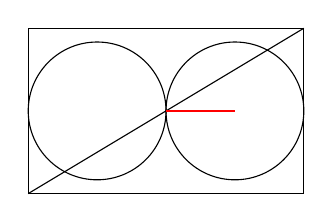
\begin{tikzpicture}[scale=0.7]
  \draw (0,0) rectangle (5,3);
  \draw (1.25,1.5) circle (1.25);
  \draw (3.75,1.5) circle (1.25);
  \draw (0,0) -- (5,3);
  \draw[red, thick] (2.5,1.5) -- (3.75,1.5);
\end{tikzpicture}
\end{center}
\vspace{1em}

\vspace{2em}
\begin{center}
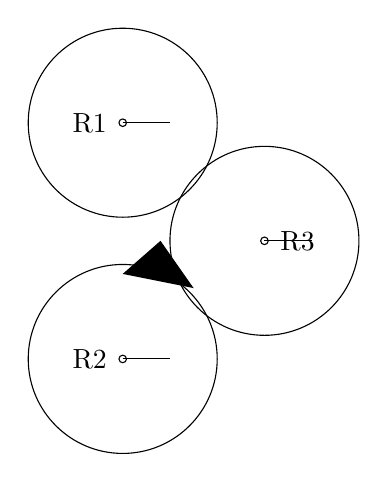
\begin{tikzpicture}[scale=0.6]
  \draw (0,2.5) circle (2);
  \draw (3,0) circle (2);
  \draw (0,-2.5) circle (2);
  \fill[black] (0.8,0) -- (0,-0.7) -- (1.5,-1) -- cycle;
  \draw (0,2.5) circle (0.08);
  \draw (3,0) circle (0.08);
  \draw (0,-2.5) circle (0.08);
  \node at (-0.7,2.5) {R1};
  \node at (3.7,0) {R3};
  \node at (-0.7,-2.5) {R2};
  \draw (0,2.5) -- ++(1,0);
  \draw (3,0) -- ++(1,0);
  \draw (0,-2.5) -- ++(1,0);
\end{tikzpicture}
\end{center}

\switchcolumn

\textbf{Closest pair of points:}

\begin{lstlisting}
struct Res {
  int64_t d;
  P a, b;
};
int64_t sq(int64_t x) { return x * x; }
int64_t dist(P &a, P &b) {
  return sq(a.x - b.x) + sq(a.y - b.y);
}
// p = py = tmp, all are same sorted by x co-ordi.;
Res closest_pair(vector<P>& p, vector<P>& py,
vector<P>& tmp, int l, int r) {
  int n = r - l + 1;
  if (n <= 1) return {LLONG_MAX, {}, {}};
  if (n == 2) {
    if (py[l].y > py[l + 1].y)
      swap(py[l], py[l + 1]);
    return {dist(p[l], p[l + 1]), p[l], p[l + 1]};
  }
  int m = (l + r) >> 1;
  int midx = p[m].x;
  Res res_l = closest_pair(p, py, tmp, l, m);
  Res res_r = closest_pair(p, py, tmp, m + 1, r);
  Res res = (res_l.d < res_r.d ? res_l : res_r);
  for (int i = l, j = m + 1, k = l; k <= r; k++) {
    if (j > r || (i <= m && py[i].y < py[j].y))
      tmp[k] = py[i++];
    else tmp[k] = py[j++];
  }
  for (int i = l; i <= r; i++) py[i] = tmp[i];
  vector<P> stripe;
  for (int i = l; i <= r; i++) {
    if (sq(py[i].x - midx) < res.d)
      stripe.push_back(py[i]);
  }
  for (int i = 0; i < (int)stripe.size(); i++) {
    for (int j = i + 1; j < (int)stripe.size(); j++) {
      if (sq(stripe[i].y - stripe[j].y) >= res.d)
        break;
      int64_t d = dist(stripe[i], stripe[j]);
      if (d < res.d) res = {d, stripe[i], stripe[j]};
    }
  }
  return res;
}
\end{lstlisting}

\begin{lstlisting}
long double L, W;
if(!(cin >> L >> W)) return 0;
// hypotenuse of each right triangle
long double h = sqrtl(L*L + W*W);
// perimeter for incenter-weights: P = L + W + h
long double P = L + W + h;
// incenter of triangle with vertices
// (0,0),(L,0),(L,W)
long double x1 = L*(L + h)/P;
long double y1 = L*W/P;
// incenter of triangle with vertices
// (0,0),(0,W),(L,W)
long double x2 = L*W/P;
long double y2 = W*(W + h)/P;
long double dx = x1 - x2;
long double dy = y1 - y2;
long double D = sqrtl(dx*dx + dy*dy);
cout << fixed << setprecision(6) << (double)D
<< "\n";
\end{lstlisting}

\begin{lstlisting}
long double r1, r2, r3;
cin >> r1 >> r2 >> r3;
// side-lengths of triangle ABC
long double a = r2 + r3;
long double b = r3 + r1;
long double c = r1 + r2;
long double s = (a + b + c) / 2.0L;
long double T = sqrtl( s*(s - a) * (s - b) * (s - c) );
// helper to compute angle opposite side a
auto angle = [&](long double opp, long double
x, long double y){
  long double cosv = (x*x + y*y - opp*opp) /
  (2.0L * x * y);
  // guard numerical drift
  cosv = min((long double)1.0, max((long
  double)-1.0, cosv));
  return acosl(cosv);
};
long double A = angle(a, b, c);
long double B = angle(b, c, a);
long double C = angle(c, a, b);
// subtract the sectors
long double sectorSum = 0.5L*(r1*r1*A +
r2*r2*B + r3*r3*C);
long double blackArea = T - sectorSum;
cout << fixed << setprecision(6) <<
(double)blackArea << "\n";
return 0;
}
\end{lstlisting}

\textbf{Intersecting Point of Two Lines Given as Pair of 2 Points}
\begin{lstlisting}
// Intersecting point of two lines (a1-a2, b1-b2)
using P = pair<ll,ll>;
auto cross = [&](P a, P b){ return
(__int128)a.first*b.second -
(__int128)a.second*b.first; };
auto intersect = [&](P a1, P a2, P b1, P b2) ->
optional<pair<long double,long double>> {
  P da = {a2.first - a1.first,
  a2.second - a1.second};
  P db = {b2.first - b1.first,
  b2.second - b1.second};
  P dc = {b1.first - a1.first,
  b1.second - a1.second};
  __int128 D = cross(da, db);
  if (!D) return {}; // parallel or coincident
  long double t = (long double)cross(dc, db) /
  (long double)D;
  return {{a1.first + da.first * t,
  a1.second + da.second * t}};
};
// Example: // if (auto p = intersect(a1,a2,b1,b2))
// cout << llround(p->first) << " " <<
// llround(p->second) << "\n";
// else
// cout << "No intersection\n";
// For segments add this before returning
long double u = (long double)cross(dc, da) / (long
double)D;
if (t < 0 || t > 1 || u < 0 || u > 1) return {};
// no segment intersection
\end{lstlisting}

\textbf{Polygon:}
\begin{lstlisting}
const ld EPS = 1e-9;
const ld PI = acos(-1.0);
int sgn(ld x) { return (x > EPS) - (x < -EPS); }
struct P {
  using T = int64_t;
  T x, y;
  void read() { cin >> x >> y; }
  P operator - (const P &b) const {
    return P{x - b.x, y - b.y}; }
  P operator + (const P &b) const {
    return P{x + b.x, y + b.y}; }
  void operator -= (const P &b) {
    x -= b.x; y -= b.y; }
  void operator += (const P &b) {
    x += b.x; y += b.y; }
  bool operator < (const P &b) const {
    return x == b.x ? y < b.y : x < b.x; }
  bool operator == (const P &b) const {
    return x == b.x && y == b.y; }
  T operator * (const P &b) const {
    return x * b.y - y * b.x; }
  T operator ^ (const P &b) const {
    return x * b.x + y * b.y; }
  T dot (P &a, P &b) const {
    return (a - *this) ^ (b - *this); }
  T cross (P &a, P &b) {
    return (a - *this) * (b - *this); }
  long double slope() {
    return (long double)y / x; }
  ld sq() const { return x * x + y * y; }
  ld abs() const { return sqrtl(sq()); }
  P rot() const { return P(-y, x); } // Rotate 90 deg CCW
  P rot(ld a) const {
    return P(x*cos(a) - y*sin(a),
    x*sin(a) + y*cos(a)); }
};
\end{lstlisting}

\begin{lstlisting}
bool collinear(P &a, P &b, P &c) {
  return (b - a) * (c - a) == 0;
}
inline bool on_segment(P &p, P &q, P &r) {
  if (!collinear(p, q, r)) return false;
  return r.x <= max(p.x, q.x) && r.x >= min(p.x,
  q.x) && r.y <= max(p.y, q.y) &&
  r.y >= min(p.y, q.y);
}
ld dist(P a, P b) { return (a - b).abs(); }
// --- Lines & Segments ---
// Project C onto line AB
P project(P a, P b, P c) {
  return a + (b - a) * (((c - a) ^ (b - a)) /
  (b - a).sq());
}
// Reflect C across line AB
P reflect(P a, P b, P c) {
  return project(a, b, c) * 2 - c;
}
// Dist from C to infinite line AB
ld dist_pt_line(P a, P b, P c) {
  return fabsl((b - a) * (c - a)) / (b - a).abs();
}
// Dist from C to segment AB
ld dist_pt_seg(P a, P b, P c) {
  if (((c - a) ^ (b - a)) <= 0) return (c - a).abs();
  if (((c - b) ^ (a - b)) <= 0) return (c - b).abs();
  return dist_pt_line(a, b, c);
}
\end{lstlisting}

\begin{lstlisting}
// Check if P is on segment AB
bool on_seg(P a, P b, P p) {
  return !sgn((b - a) * (p - a)) &&
  ((p - a) ^ (p - b)) <= EPS;
}
// Line-Line Intersection (returns false if parallel)
bool line_int(P a, P b, P c, P d, P &res) {
  ld cp = (b - a) * (d - c);
  if (!sgn(cp)) return false;
  res = a + (b - a) * (((d - c) * (c - a)) / cp);
  return true;
}
// Segment-Segment Intersection
bool seg_int(P a, P b, P c, P d) {
  auto cp = [&](P x, P y, P z) {
    return sgn((y - x) * (z - x)); };
  if (on_seg(a, b, c) || on_seg(a, b, d) ||
  on_seg(c, d, a) || on_seg(c, d, b)) return true;
  return cp(a, b, c) != cp(a, b, d) &&
  cp(c, d, a) != cp(c, d, b);
}
long double polygon_area(vector<P> &p) {
  int64_t area = 0, n = p.size();
  for (int i = 0; i < n; ++i)
    area += p[i] * p[(i + 1) % n];
  return abs(area) / 2;
}
\end{lstlisting}

\begin{lstlisting}
vector<P> convexHull(vector<P> p) {
  int n = p.size(), k = 0;
  if (n <= 2) return p;
  vector<P> h(2 * n);
  sort(p.begin(), p.end());
  for (int i = 0; i < n; h[k++] = p[i++])
    while (k >= 2 && h[k - 2].cross(h[k - 1],
    p[i]) <= 0) k--;
  for (int i = n - 2, t = k + 1; i >= 0;
  h[k++] = p[i--])
    while (k >= t && h[k - 2].cross(h[k - 1],
    p[i]) <= 0) k--;
  h.resize(k - 1);
  return h;
}
int is_point_in_polygon(const vector<P>& p, P
q) {
  int c = 0;
  for (int i = 0, n = p.size(); i < n; ++i) {
    P a = p[i], b = p[(i + 1) % n];
    if ((b - a) * (q - a) == 0 && min(a.x, b.x) <= q.x
    && q.x <= max(a.x, b.x) && min(a.y, b.y) <= q.y
    && q.y <= max(a.y, b.y)) return 2;
    if ((a.y > q.y) != (b.y > q.y) &&
    ((b - a) * (q - a) > 0) == (a.y < b.y))
      c = !c;
  }
  return c;
}
double angle_at_vertex(P &a, P &b, P &c) {
  double ang_rad = atan2l(fabs(b.cross(a, c)),
  b.dot(a, c));
  return ang_rad * 180.0L / acosl(-1.0L);
}
ld dist_point_line(P a, P b, P c) {
  ld area2 = fabsl((b - a) * (c - a));
  ld base = hypotl(b.x - a.x, b.y - a.y);
  return area2 / base;
}
\end{lstlisting}

\textbf{MO:}
\begin{lstlisting}
sort(cu.begin(), cu.end(), [&](auto &x, auto &y){
  if (x.l / B != y.l / B) return x.l / B < y.l / B;
  return (x.l / B) % 2 ? x.r > y.r : x.r < y.r;
});
int R = -1, L = 0;
while (R < r) add(++R);
while (L > l) add(--L);
while (R > r) rem(R--);
while (L < l) rem(L++);
\end{lstlisting}

\textbf{Fast Factorization (Maybe not prime)}
\begin{lstlisting}
#define ull uint64_t
struct Montgomery {
  ull n, nr;
  Montgomery(ull n) {
    this->n = n, nr = 1;
    for (int i = 0; i < 6; i++)
      nr *= 2 - n * nr;
  }
  ull reduce(__uint128_t x) const {
    ull q = ull(x) * nr,
    m = ((__uint128_t)q * n) >> 64;
    return (x >> 64) + n - m;
  }
  ull multiply(ull x, ull y) {
    return reduce((__uint128_t)x * y); }
};
ull f(ull x, Montgomery& m, ull a) {
  return m.multiply(x, x) + a; }
ull diff(ull a, ull b) {
  return a > b ? a - b : b - a; }
const int M = 1024;
const ull SEED = 42;
ull find_factor(ull n, ull x0 = 2, ull a = 1)
{
  Montgomery m(n);
  ull x = SEED;
  for (int l = M; l < (1 << 20); l *= 2) {
    ull y = x, p = 1;
    for (int i = 0; i < l; i += M) {
      for (int j = 0; j < M; j++)
        x = f(x, m, a), p = m.multiply(p,
        diff(x, y));
      if (ull g = gcd(p, n); g != 1)
        return g;
    }
  }
  return n;
}
int32_t main() {
  ll n;
  cin >> n;
  ll factor = find_factor(n);
  if (factor != 1) {
    cout << "Factor found: " << factor << endl;
  } else {
    cout << "No factor found" << endl;
  }
  return 0;
}
\end{lstlisting}

OR convolution = SOS DP

\end{paracol}
\end{document}
